\documentclass[1p]{elsarticle_modified}
%\bibliographystyle{elsarticle-num}

%\usepackage[colorlinks]{hyperref}
%\usepackage{abbrmath_seonhwa} %\Abb, \Ascr, \Acal ,\Abf, \Afrak
\usepackage{amsfonts}
\usepackage{amssymb}
\usepackage{amsmath}
\usepackage{amsthm}
\usepackage{scalefnt}
\usepackage{amsbsy}
\usepackage{kotex}
\usepackage{caption}
\usepackage{subfig}
\usepackage{color}
\usepackage{graphicx}
\usepackage{xcolor} %% white, black, red, green, blue, cyan, magenta, yellow
\usepackage{float}
\usepackage{setspace}
\usepackage{hyperref}

\usepackage{tikz}
\usetikzlibrary{arrows}

\usepackage{multirow}
\usepackage{array} % fixed length table
\usepackage{hhline}

%%%%%%%%%%%%%%%%%%%%%
\makeatletter
\renewcommand*\env@matrix[1][\arraystretch]{%
	\edef\arraystretch{#1}%
	\hskip -\arraycolsep
	\let\@ifnextchar\new@ifnextchar
	\array{*\c@MaxMatrixCols c}}
\makeatother %https://tex.stackexchange.com/questions/14071/how-can-i-increase-the-line-spacing-in-a-matrix
%%%%%%%%%%%%%%%

\usepackage[normalem]{ulem}

\newcommand{\msout}[1]{\ifmmode\text{\sout{\ensuremath{#1}}}\else\sout{#1}\fi}
%SOURCE: \msout is \stkout macro in https://tex.stackexchange.com/questions/20609/strikeout-in-math-mode

\newcommand{\cancel}[1]{
	\ifmmode
	{\color{red}\msout{#1}}
	\else
	{\color{red}\sout{#1}}
	\fi
}

\newcommand{\add}[1]{
	{\color{blue}\uwave{#1}}
}

\newcommand{\replace}[2]{
	\ifmmode
	{\color{red}\msout{#1}}{\color{blue}\uwave{#2}}
	\else
	{\color{red}\sout{#1}}{\color{blue}\uwave{#2}}
	\fi
}

\newcommand{\Sol}{\mathcal{S}} %segment
\newcommand{\D}{D} %diagram
\newcommand{\A}{\mathcal{A}} %arc


%%%%%%%%%%%%%%%%%%%%%%%%%%%%%5 test

\def\sl{\operatorname{\textup{SL}}(2,\Cbb)}
\def\psl{\operatorname{\textup{PSL}}(2,\Cbb)}
\def\quan{\mkern 1mu \triangleright \mkern 1mu}

\theoremstyle{definition}
\newtheorem{thm}{Theorem}[section]
\newtheorem{prop}[thm]{Proposition}
\newtheorem{lem}[thm]{Lemma}
\newtheorem{ques}[thm]{Question}
\newtheorem{cor}[thm]{Corollary}
\newtheorem{defn}[thm]{Definition}
\newtheorem{exam}[thm]{Example}
\newtheorem{rmk}[thm]{Remark}
\newtheorem{alg}[thm]{Algorithm}

\newcommand{\I}{\sqrt{-1}}
\begin{document}

%\begin{frontmatter}
%
%\title{Boundary parabolic representations of knots up to 8 crossings}
%
%%% Group authors per affiliation:
%\author{Yunhi Cho} 
%\address{Department of Mathematics, University of Seoul, Seoul, Korea}
%\ead{yhcho@uos.ac.kr}
%
%
%\author{Seonhwa Kim} %\fnref{s_kim}}
%\address{Center for Geometry and Physics, Institute for Basic Science, Pohang, 37673, Korea}
%\ead{ryeona17@ibs.re.kr}
%
%\author{Hyuk Kim}
%\address{Department of Mathematical Sciences, Seoul National University, Seoul 08826, Korea}
%\ead{hyukkim@snu.ac.kr}
%
%\author{Seokbeom Yoon}
%\address{Department of Mathematical Sciences, Seoul National University, Seoul, 08826,  Korea}
%\ead{sbyoon15@snu.ac.kr}
%
%\begin{abstract}
%We find all boundary parabolic representation of knots up to 8 crossings.
%
%\end{abstract}
%\begin{keyword}
%    \MSC[2010] 57M25 
%\end{keyword}
%
%\end{frontmatter}

%\linenumbers
%\tableofcontents
%
\newcommand\colored[1]{\textcolor{white}{\rule[-0.35ex]{0.8em}{1.4ex}}\kern-0.8em\color{red} #1}%
%\newcommand\colored[1]{\textcolor{white}{ #1}\kern-2.17ex	\textcolor{white}{ #1}\kern-1.81ex	\textcolor{white}{ #1}\kern-2.15ex\color{red}#1	}

{\Large $\underline{12a_{1133}~(K12a_{1133})}$}

\setlength{\tabcolsep}{10pt}
\renewcommand{\arraystretch}{1.6}
\vspace{1cm}\begin{tabular}{m{100pt}>{\centering\arraybackslash}m{274pt}}
\multirow{5}{120pt}{
	\centering
	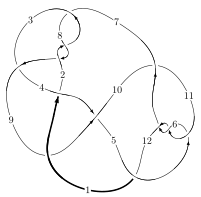
\includegraphics[width=112pt]{../../../GIT/diagram.site/Diagrams/png/1934_12a_1133.png}\\
\ \ \ A knot diagram\footnotemark}&
\allowdisplaybreaks
\textbf{Linearized knot diagam} \\
\cline{2-2}
 &
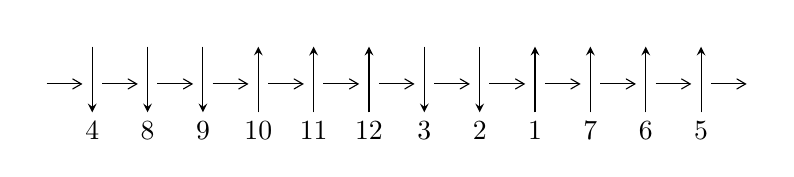
\begin{tikzpicture}[x=20pt, y=17pt]
	% nodes
	\node (C0) at (0, 0) {};
	\node (C1) at (1, 0) {};
	\node (C1U) at (1, +1) {};
	\node (C1D) at (1, -1) {4};

	\node (C2) at (2, 0) {};
	\node (C2U) at (2, +1) {};
	\node (C2D) at (2, -1) {8};

	\node (C3) at (3, 0) {};
	\node (C3U) at (3, +1) {};
	\node (C3D) at (3, -1) {9};

	\node (C4) at (4, 0) {};
	\node (C4U) at (4, +1) {};
	\node (C4D) at (4, -1) {10};

	\node (C5) at (5, 0) {};
	\node (C5U) at (5, +1) {};
	\node (C5D) at (5, -1) {11};

	\node (C6) at (6, 0) {};
	\node (C6U) at (6, +1) {};
	\node (C6D) at (6, -1) {12};

	\node (C7) at (7, 0) {};
	\node (C7U) at (7, +1) {};
	\node (C7D) at (7, -1) {3};

	\node (C8) at (8, 0) {};
	\node (C8U) at (8, +1) {};
	\node (C8D) at (8, -1) {2};

	\node (C9) at (9, 0) {};
	\node (C9U) at (9, +1) {};
	\node (C9D) at (9, -1) {1};

	\node (C10) at (10, 0) {};
	\node (C10U) at (10, +1) {};
	\node (C10D) at (10, -1) {7};

	\node (C11) at (11, 0) {};
	\node (C11U) at (11, +1) {};
	\node (C11D) at (11, -1) {6};

	\node (C12) at (12, 0) {};
	\node (C12U) at (12, +1) {};
	\node (C12D) at (12, -1) {5};
	\node (C13) at (13, 0) {};

	% arrows
	\draw[->,>={angle 60}]
	(C0) edge (C1) (C1) edge (C2) (C2) edge (C3) (C3) edge (C4) (C4) edge (C5) (C5) edge (C6) (C6) edge (C7) (C7) edge (C8) (C8) edge (C9) (C9) edge (C10) (C10) edge (C11) (C11) edge (C12) (C12) edge (C13) ;	\draw[->,>=stealth]
	(C1U) edge (C1D) (C2U) edge (C2D) (C3U) edge (C3D) (C4D) edge (C4U) (C5D) edge (C5U) (C6D) edge (C6U) (C7U) edge (C7D) (C8U) edge (C8D) (C9D) edge (C9U) (C10D) edge (C10U) (C11D) edge (C11U) (C12D) edge (C12U) ;
	\end{tikzpicture} \\
\hhline{~~} \\& 
\textbf{Solving Sequence} \\ \cline{2-2} 
 &
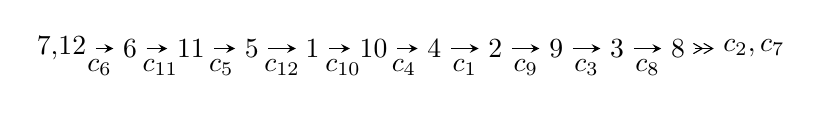
\begin{tikzpicture}[x=22pt, y=7pt]
	% node
	\node (A0) at (-1/8, 0) {7,12};
	\node (A1) at (1, 0) {6};
	\node (A2) at (2, 0) {11};
	\node (A3) at (3, 0) {5};
	\node (A4) at (4, 0) {1};
	\node (A5) at (5, 0) {10};
	\node (A6) at (6, 0) {4};
	\node (A7) at (7, 0) {2};
	\node (A8) at (8, 0) {9};
	\node (A9) at (9, 0) {3};
	\node (A10) at (10, 0) {8};
	\node (C1) at (1/2, -1) {$c_{6}$};
	\node (C2) at (3/2, -1) {$c_{11}$};
	\node (C3) at (5/2, -1) {$c_{5}$};
	\node (C4) at (7/2, -1) {$c_{12}$};
	\node (C5) at (9/2, -1) {$c_{10}$};
	\node (C6) at (11/2, -1) {$c_{4}$};
	\node (C7) at (13/2, -1) {$c_{1}$};
	\node (C8) at (15/2, -1) {$c_{9}$};
	\node (C9) at (17/2, -1) {$c_{3}$};
	\node (C10) at (19/2, -1) {$c_{8}$};
	\node (A11) at (45/4, 0) {$c_{2},c_{7}$};

	% edge
	\draw[->,>=stealth]	
	(A0) edge (A1) (A1) edge (A2) (A2) edge (A3) (A3) edge (A4) (A4) edge (A5) (A5) edge (A6) (A6) edge (A7) (A7) edge (A8) (A8) edge (A9) (A9) edge (A10) ;
	\draw[->>,>={angle 60}]	
	(A10) edge (A11);
\end{tikzpicture} \\ 

\end{tabular} \\

\footnotetext{
The image of knot diagram is generated by the software ``\textbf{Draw programme}" developed by Andrew Bartholomew(\url{http://www.layer8.co.uk/maths/draw/index.htm\#Running-draw}), where we modified some parts for our purpose(\url{https://github.com/CATsTAILs/LinksPainter}).
}\phantom \\ \newline 
\centering \textbf{Ideals for irreducible components\footnotemark of $X_{\text{par}}$} 
 
\begin{align*}
I^u_{1}&=\langle 
u^{79}- u^{78}+\cdots+2 u+1\rangle \\
\\
\end{align*}
\raggedright * 1 irreducible components of $\dim_{\mathbb{C}}=0$, with total 79 representations.\\
\footnotetext{All coefficients of polynomials are rational numbers. But the coefficients are sometimes approximated in decimal forms when there is not enough margin.}
\newpage
\renewcommand{\arraystretch}{1}
\centering \section*{I. $I^u_{1}= \langle u^{79}- u^{78}+\cdots+2 u+1 \rangle$}
\flushleft \textbf{(i) Arc colorings}\\
\begin{tabular}{m{7pt} m{180pt} m{7pt} m{180pt} }
\flushright $a_{7}=$&$\begin{pmatrix}1\\0\end{pmatrix}$ \\
\flushright $a_{12}=$&$\begin{pmatrix}0\\u\end{pmatrix}$ \\
\flushright $a_{6}=$&$\begin{pmatrix}1\\u^2\end{pmatrix}$ \\
\flushright $a_{11}=$&$\begin{pmatrix}- u\\- u^3+u\end{pmatrix}$ \\
\flushright $a_{5}=$&$\begin{pmatrix}- u^2+1\\- u^4+2 u^2\end{pmatrix}$ \\
\flushright $a_{1}=$&$\begin{pmatrix}u^5-2 u^3+u\\u^7-3 u^5+2 u^3+u\end{pmatrix}$ \\
\flushright $a_{10}=$&$\begin{pmatrix}u^3-2 u\\- u^3+u\end{pmatrix}$ \\
\flushright $a_{4}=$&$\begin{pmatrix}u^{10}-5 u^8+8 u^6-3 u^4-3 u^2+1\\- u^{10}+4 u^8-5 u^6+3 u^2\end{pmatrix}$ \\
\flushright $a_{2}=$&$\begin{pmatrix}- u^{27}+12 u^{25}+\cdots-2 u^5+5 u^3\\u^{27}-11 u^{25}+\cdots- u^3+u\end{pmatrix}$ \\
\flushright $a_{9}=$&$\begin{pmatrix}u^{15}-6 u^{13}+14 u^{11}-14 u^9+2 u^7+6 u^5-2 u^3-2 u\\u^{17}-7 u^{15}+19 u^{13}-22 u^{11}+3 u^9+14 u^7-6 u^5-4 u^3+u\end{pmatrix}$ \\
\flushright $a_{3}=$&$\begin{pmatrix}- u^{42}+17 u^{40}+\cdots- u^2+1\\- u^{44}+18 u^{42}+\cdots+5 u^4+2 u^2\end{pmatrix}$ \\
\flushright $a_{8}=$&$\begin{pmatrix}u^{71}-30 u^{69}+\cdots-2 u^3-2 u\\- u^{71}+29 u^{69}+\cdots-2 u^3+u\end{pmatrix}$\\&\end{tabular}
\flushleft \textbf{(ii) Obstruction class $= -1$}\\~\\
\flushleft \textbf{(iii) Cusp Shapes $= -4 u^{77}+128 u^{75}+\cdots+16 u+10$}\\~\\
\newpage\renewcommand{\arraystretch}{1}
\flushleft \textbf{(iv) u-Polynomials at the component}\newline \\
\begin{tabular}{m{50pt}|m{274pt}}
Crossings & \hspace{64pt}u-Polynomials at each crossing \\
\hline $$\begin{aligned}c_{1}\end{aligned}$$&$\begin{aligned}
&u^{79}-17 u^{78}+\cdots-26040 u+1697
\end{aligned}$\\
\hline $$\begin{aligned}c_{2},c_{7},c_{8}\end{aligned}$$&$\begin{aligned}
&u^{79}- u^{78}+\cdots+2 u-1
\end{aligned}$\\
\hline $$\begin{aligned}c_{3}\end{aligned}$$&$\begin{aligned}
&u^{79}+u^{78}+\cdots+13 u-2
\end{aligned}$\\
\hline $$\begin{aligned}c_{4}\end{aligned}$$&$\begin{aligned}
&u^{79}- u^{78}+\cdots-40 u-25
\end{aligned}$\\
\hline $$\begin{aligned}c_{5},c_{6},c_{11}\end{aligned}$$&$\begin{aligned}
&u^{79}+u^{78}+\cdots+2 u-1
\end{aligned}$\\
\hline $$\begin{aligned}c_{9}\end{aligned}$$&$\begin{aligned}
&u^{79}-7 u^{78}+\cdots+4620 u+121
\end{aligned}$\\
\hline $$\begin{aligned}c_{10},c_{12}\end{aligned}$$&$\begin{aligned}
&u^{79}-3 u^{78}+\cdots-221 u+56
\end{aligned}$\\
\hline
\end{tabular}\\~\\
\newpage\renewcommand{\arraystretch}{1}
\flushleft \textbf{(v) Riley Polynomials at the component}\newline \\
\begin{tabular}{m{50pt}|m{274pt}}
Crossings & \hspace{64pt}Riley Polynomials at each crossing \\
\hline $$\begin{aligned}c_{1}\end{aligned}$$&$\begin{aligned}
&y^{79}+23 y^{78}+\cdots-69562296 y-2879809
\end{aligned}$\\
\hline $$\begin{aligned}c_{2},c_{7},c_{8}\end{aligned}$$&$\begin{aligned}
&y^{79}+71 y^{78}+\cdots-8 y^2-1
\end{aligned}$\\
\hline $$\begin{aligned}c_{3}\end{aligned}$$&$\begin{aligned}
&y^{79}+3 y^{78}+\cdots-11 y-4
\end{aligned}$\\
\hline $$\begin{aligned}c_{4}\end{aligned}$$&$\begin{aligned}
&y^{79}-5 y^{78}+\cdots+34200 y-625
\end{aligned}$\\
\hline $$\begin{aligned}c_{5},c_{6},c_{11}\end{aligned}$$&$\begin{aligned}
&y^{79}-65 y^{78}+\cdots-4 y^2-1
\end{aligned}$\\
\hline $$\begin{aligned}c_{9}\end{aligned}$$&$\begin{aligned}
&y^{79}+19 y^{78}+\cdots+25448720 y-14641
\end{aligned}$\\
\hline $$\begin{aligned}c_{10},c_{12}\end{aligned}$$&$\begin{aligned}
&y^{79}+51 y^{78}+\cdots+22297 y-3136
\end{aligned}$\\
\hline
\end{tabular}\\~\\
\newpage\flushleft \textbf{(vi) Complex Volumes and Cusp Shapes}
$$\begin{array}{c|c|c}  
\text{Solutions to }I^u_{1}& \I (\text{vol} + \sqrt{-1}CS) & \text{Cusp shape}\\
 \hline 
\begin{aligned}
u &= \phantom{-}1.119910 + 0.269996 I\end{aligned}
 & \phantom{-}6.31309 + 1.50449 I & \phantom{-0.000000 } 0 \\ \hline\begin{aligned}
u &= \phantom{-}1.119910 - 0.269996 I\end{aligned}
 & \phantom{-}6.31309 - 1.50449 I & \phantom{-0.000000 } 0 \\ \hline\begin{aligned}
u &= -1.116140 + 0.344098 I\end{aligned}
 & \phantom{-}3.99592 + 7.01460 I & \phantom{-0.000000 } 0 \\ \hline\begin{aligned}
u &= -1.116140 - 0.344098 I\end{aligned}
 & \phantom{-}3.99592 - 7.01460 I & \phantom{-0.000000 } 0 \\ \hline\begin{aligned}
u &= \phantom{-}1.129450 + 0.339661 I\end{aligned}
 & -1.35951 - 3.44188 I & \phantom{-0.000000 } 0 \\ \hline\begin{aligned}
u &= \phantom{-}1.129450 - 0.339661 I\end{aligned}
 & -1.35951 + 3.44188 I & \phantom{-0.000000 } 0 \\ \hline\begin{aligned}
u &= -0.127859 + 0.804619 I\end{aligned}
 & \phantom{-}0.99138 - 11.20740 I & \phantom{-}1.90900 + 7.76695 I \\ \hline\begin{aligned}
u &= -0.127859 - 0.804619 I\end{aligned}
 & \phantom{-}0.99138 + 11.20740 I & \phantom{-}1.90900 - 7.76695 I \\ \hline\begin{aligned}
u &= \phantom{-}0.120290 + 0.801749 I\end{aligned}
 & -4.42516 + 7.60535 I & -2.69052 - 7.48919 I \\ \hline\begin{aligned}
u &= \phantom{-}0.120290 - 0.801749 I\end{aligned}
 & -4.42516 - 7.60535 I & -2.69052 + 7.48919 I \\ \hline\begin{aligned}
u &= -1.151830 + 0.322827 I\end{aligned}
 & \phantom{-}0.174975 - 0.262644 I & \phantom{-0.000000 } 0 \\ \hline\begin{aligned}
u &= -1.151830 - 0.322827 I\end{aligned}
 & \phantom{-}0.174975 + 0.262644 I & \phantom{-0.000000 } 0 \\ \hline\begin{aligned}
u &= -0.088144 + 0.798068 I\end{aligned}
 & -3.42247 - 4.03212 I & -1.76280 + 4.49310 I \\ \hline\begin{aligned}
u &= -0.088144 - 0.798068 I\end{aligned}
 & -3.42247 + 4.03212 I & -1.76280 - 4.49310 I \\ \hline\begin{aligned}
u &= -0.046884 + 0.799298 I\end{aligned}
 & -1.44028 + 2.80439 I & -0.85617 - 2.18147 I \\ \hline\begin{aligned}
u &= -0.046884 - 0.799298 I\end{aligned}
 & -1.44028 - 2.80439 I & -0.85617 + 2.18147 I \\ \hline\begin{aligned}
u &= \phantom{-}0.065230 + 0.795734 I\end{aligned}
 & -6.12113 + 0.61604 I & -6.03236 + 0.34847 I \\ \hline\begin{aligned}
u &= \phantom{-}0.065230 - 0.795734 I\end{aligned}
 & -6.12113 - 0.61604 I & -6.03236 - 0.34847 I \\ \hline\begin{aligned}
u &= -0.109674 + 0.789656 I\end{aligned}
 & -2.98096 - 3.79614 I & -0.06060 + 2.39804 I \\ \hline\begin{aligned}
u &= -0.109674 - 0.789656 I\end{aligned}
 & -2.98096 + 3.79614 I & -0.06060 - 2.39804 I \\ \hline\begin{aligned}
u &= \phantom{-}0.129454 + 0.770426 I\end{aligned}
 & \phantom{-}3.35446 + 2.37248 I & \phantom{-}4.39926 - 2.88601 I \\ \hline\begin{aligned}
u &= \phantom{-}0.129454 - 0.770426 I\end{aligned}
 & \phantom{-}3.35446 - 2.37248 I & \phantom{-}4.39926 + 2.88601 I \\ \hline\begin{aligned}
u &= -1.174720 + 0.339826 I\end{aligned}
 & -0.109212 - 0.094646 I & \phantom{-0.000000 } 0 \\ \hline\begin{aligned}
u &= -1.174720 - 0.339826 I\end{aligned}
 & -0.109212 + 0.094646 I & \phantom{-0.000000 } 0 \\ \hline\begin{aligned}
u &= \phantom{-}1.201820 + 0.343577 I\end{aligned}
 & -2.63933 + 3.50252 I & \phantom{-0.000000 } 0 \\ \hline\begin{aligned}
u &= \phantom{-}1.201820 - 0.343577 I\end{aligned}
 & -2.63933 - 3.50252 I & \phantom{-0.000000 } 0 \\ \hline\begin{aligned}
u &= -1.217970 + 0.349990 I\end{aligned}
 & \phantom{-}2.16029 - 6.95203 I & \phantom{-0.000000 } 0 \\ \hline\begin{aligned}
u &= -1.217970 - 0.349990 I\end{aligned}
 & \phantom{-}2.16029 + 6.95203 I & \phantom{-0.000000 } 0 \\ \hline\begin{aligned}
u &= -1.27536\phantom{ +0.000000I}\end{aligned}
 & \phantom{-}2.83534\phantom{ +0.000000I} & \phantom{-0.000000 } 0 \\ \hline\begin{aligned}
u &= \phantom{-}1.318290 + 0.071541 I\end{aligned}
 & \phantom{-}6.31838 + 2.66253 I & \phantom{-0.000000 } 0\\
 \hline 
 \end{array}$$\newpage$$\begin{array}{c|c|c}  
\text{Solutions to }I^u_{1}& \I (\text{vol} + \sqrt{-1}CS) & \text{Cusp shape}\\
 \hline 
\begin{aligned}
u &= \phantom{-}1.318290 - 0.071541 I\end{aligned}
 & \phantom{-}6.31838 - 2.66253 I & \phantom{-0.000000 } 0 \\ \hline\begin{aligned}
u &= -1.311270 + 0.248102 I\end{aligned}
 & \phantom{-}3.39241 - 1.40885 I & \phantom{-0.000000 } 0 \\ \hline\begin{aligned}
u &= -1.311270 - 0.248102 I\end{aligned}
 & \phantom{-}3.39241 + 1.40885 I & \phantom{-0.000000 } 0 \\ \hline\begin{aligned}
u &= \phantom{-}1.296480 + 0.346961 I\end{aligned}
 & \phantom{-}2.75060 + 1.32326 I & \phantom{-0.000000 } 0 \\ \hline\begin{aligned}
u &= \phantom{-}1.296480 - 0.346961 I\end{aligned}
 & \phantom{-}2.75060 - 1.32326 I & \phantom{-0.000000 } 0 \\ \hline\begin{aligned}
u &= \phantom{-}0.156652 + 0.634430 I\end{aligned}
 & \phantom{-}5.00375 + 3.99260 I & \phantom{-}5.33060 - 4.90046 I \\ \hline\begin{aligned}
u &= \phantom{-}0.156652 - 0.634430 I\end{aligned}
 & \phantom{-}5.00375 - 3.99260 I & \phantom{-}5.33060 + 4.90046 I \\ \hline\begin{aligned}
u &= \phantom{-}1.320350 + 0.276038 I\end{aligned}
 & \phantom{-}3.78685 + 4.88557 I & \phantom{-0.000000 } 0 \\ \hline\begin{aligned}
u &= \phantom{-}1.320350 - 0.276038 I\end{aligned}
 & \phantom{-}3.78685 - 4.88557 I & \phantom{-0.000000 } 0 \\ \hline\begin{aligned}
u &= \phantom{-}1.330100 + 0.236506 I\end{aligned}
 & \phantom{-}8.98594 - 1.62355 I & \phantom{-0.000000 } 0 \\ \hline\begin{aligned}
u &= \phantom{-}1.330100 - 0.236506 I\end{aligned}
 & \phantom{-}8.98594 + 1.62355 I & \phantom{-0.000000 } 0 \\ \hline\begin{aligned}
u &= -1.310030 + 0.345318 I\end{aligned}
 & -1.81920 - 4.72773 I & \phantom{-0.000000 } 0 \\ \hline\begin{aligned}
u &= -1.310030 - 0.345318 I\end{aligned}
 & -1.81920 + 4.72773 I & \phantom{-0.000000 } 0 \\ \hline\begin{aligned}
u &= -0.543300 + 0.338999 I\end{aligned}
 & \phantom{-}5.11761 - 7.49924 I & \phantom{-}6.46948 + 7.99126 I \\ \hline\begin{aligned}
u &= -0.543300 - 0.338999 I\end{aligned}
 & \phantom{-}5.11761 + 7.49924 I & \phantom{-}6.46948 - 7.99126 I \\ \hline\begin{aligned}
u &= \phantom{-}0.601727 + 0.206736 I\end{aligned}
 & \phantom{-}6.71860 - 1.01423 I & \phantom{-}9.60570 - 1.23872 I \\ \hline\begin{aligned}
u &= \phantom{-}0.601727 - 0.206736 I\end{aligned}
 & \phantom{-}6.71860 + 1.01423 I & \phantom{-}9.60570 + 1.23872 I \\ \hline\begin{aligned}
u &= -1.339530 + 0.276387 I\end{aligned}
 & \phantom{-}9.68534 - 7.36202 I & \phantom{-0.000000 } 0 \\ \hline\begin{aligned}
u &= -1.339530 - 0.276387 I\end{aligned}
 & \phantom{-}9.68534 + 7.36202 I & \phantom{-0.000000 } 0 \\ \hline\begin{aligned}
u &= \phantom{-}1.324120 + 0.346948 I\end{aligned}
 & \phantom{-}1.00559 + 8.16070 I & \phantom{-0.000000 } 0 \\ \hline\begin{aligned}
u &= \phantom{-}1.324120 - 0.346948 I\end{aligned}
 & \phantom{-}1.00559 - 8.16070 I & \phantom{-0.000000 } 0 \\ \hline\begin{aligned}
u &= \phantom{-}1.369290 + 0.043682 I\end{aligned}
 & \phantom{-}6.62983 + 1.55922 I & \phantom{-0.000000 } 0 \\ \hline\begin{aligned}
u &= \phantom{-}1.369290 - 0.043682 I\end{aligned}
 & \phantom{-}6.62983 - 1.55922 I & \phantom{-0.000000 } 0 \\ \hline\begin{aligned}
u &= -0.080168 + 0.624756 I\end{aligned}
 & -0.62665 - 1.53685 I & \phantom{-}1.09952 + 5.24112 I \\ \hline\begin{aligned}
u &= -0.080168 - 0.624756 I\end{aligned}
 & -0.62665 + 1.53685 I & \phantom{-}1.09952 - 5.24112 I \\ \hline\begin{aligned}
u &= \phantom{-}1.337040 + 0.341010 I\end{aligned}
 & \phantom{-}1.56661 + 7.87869 I & \phantom{-0.000000 } 0 \\ \hline\begin{aligned}
u &= \phantom{-}1.337040 - 0.341010 I\end{aligned}
 & \phantom{-}1.56661 - 7.87869 I & \phantom{-0.000000 } 0 \\ \hline\begin{aligned}
u &= -1.379070 + 0.061269 I\end{aligned}
 & \phantom{-}5.59871 - 5.23109 I & \phantom{-0.000000 } 0 \\ \hline\begin{aligned}
u &= -1.379070 - 0.061269 I\end{aligned}
 & \phantom{-}5.59871 + 5.23109 I & \phantom{-0.000000 } 0 \\ \hline\begin{aligned}
u &= -1.344960 + 0.330309 I\end{aligned}
 & \phantom{-}7.99521 - 6.35631 I & \phantom{-0.000000 } 0\\
 \hline 
 \end{array}$$\newpage$$\begin{array}{c|c|c}  
\text{Solutions to }I^u_{1}& \I (\text{vol} + \sqrt{-1}CS) & \text{Cusp shape}\\
 \hline 
\begin{aligned}
u &= -1.344960 - 0.330309 I\end{aligned}
 & \phantom{-}7.99521 + 6.35631 I & \phantom{-0.000000 } 0 \\ \hline\begin{aligned}
u &= -1.343360 + 0.346682 I\end{aligned}
 & \phantom{-}0.17815 - 11.74890 I & \phantom{-0.000000 } 0 \\ \hline\begin{aligned}
u &= -1.343360 - 0.346682 I\end{aligned}
 & \phantom{-}0.17815 + 11.74890 I & \phantom{-0.000000 } 0 \\ \hline\begin{aligned}
u &= -1.387760 + 0.032369 I\end{aligned}
 & \phantom{-}12.77490 + 0.40459 I & \phantom{-0.000000 } 0 \\ \hline\begin{aligned}
u &= -1.387760 - 0.032369 I\end{aligned}
 & \phantom{-}12.77490 - 0.40459 I & \phantom{-0.000000 } 0 \\ \hline\begin{aligned}
u &= \phantom{-}1.389120 + 0.063240 I\end{aligned}
 & \phantom{-}11.12760 + 8.64852 I & \phantom{-0.000000 } 0 \\ \hline\begin{aligned}
u &= \phantom{-}1.389120 - 0.063240 I\end{aligned}
 & \phantom{-}11.12760 - 8.64852 I & \phantom{-0.000000 } 0 \\ \hline\begin{aligned}
u &= \phantom{-}1.347730 + 0.347472 I\end{aligned}
 & \phantom{-}5.6350 + 15.3639 I & \phantom{-0.000000 } 0 \\ \hline\begin{aligned}
u &= \phantom{-}1.347730 - 0.347472 I\end{aligned}
 & \phantom{-}5.6350 - 15.3639 I & \phantom{-0.000000 } 0 \\ \hline\begin{aligned}
u &= \phantom{-}0.508944 + 0.322602 I\end{aligned}
 & -0.25179 + 4.12095 I & \phantom{-}1.80082 - 8.29426 I \\ \hline\begin{aligned}
u &= \phantom{-}0.508944 - 0.322602 I\end{aligned}
 & -0.25179 - 4.12095 I & \phantom{-}1.80082 + 8.29426 I \\ \hline\begin{aligned}
u &= -0.252272 + 0.515953 I\end{aligned}
 & \phantom{-}4.20461 + 4.40403 I & \phantom{-}4.02126 - 1.02784 I \\ \hline\begin{aligned}
u &= -0.252272 - 0.515953 I\end{aligned}
 & \phantom{-}4.20461 - 4.40403 I & \phantom{-}4.02126 + 1.02784 I \\ \hline\begin{aligned}
u &= -0.466798 + 0.223035 I\end{aligned}
 & \phantom{-}0.965294 - 0.777908 I & \phantom{-}6.33896 + 2.42905 I \\ \hline\begin{aligned}
u &= -0.466798 - 0.223035 I\end{aligned}
 & \phantom{-}0.965294 + 0.777908 I & \phantom{-}6.33896 - 2.42905 I \\ \hline\begin{aligned}
u &= -0.373663 + 0.351639 I\end{aligned}
 & \phantom{-}1.20042 - 1.33503 I & \phantom{-}2.25607 + 5.14188 I \\ \hline\begin{aligned}
u &= -0.373663 - 0.351639 I\end{aligned}
 & \phantom{-}1.20042 + 1.33503 I & \phantom{-}2.25607 - 5.14188 I \\ \hline\begin{aligned}
u &= \phantom{-}0.237055 + 0.443394 I\end{aligned}
 & -1.04518 - 1.27519 I & -1.51740 + 0.90528 I \\ \hline\begin{aligned}
u &= \phantom{-}0.237055 - 0.443394 I\end{aligned}
 & -1.04518 + 1.27519 I & -1.51740 - 0.90528 I\\
 \hline 
 \end{array}$$\newpage
\newpage\renewcommand{\arraystretch}{1}
\centering \section*{ II. u-Polynomials}
\begin{tabular}{m{50pt}|m{274pt}}
Crossings & \hspace{64pt}u-Polynomials at each crossing \\
\hline $$\begin{aligned}c_{1}\end{aligned}$$&$\begin{aligned}
&u^{79}-17 u^{78}+\cdots-26040 u+1697
\end{aligned}$\\
\hline $$\begin{aligned}c_{2},c_{7},c_{8}\end{aligned}$$&$\begin{aligned}
&u^{79}- u^{78}+\cdots+2 u-1
\end{aligned}$\\
\hline $$\begin{aligned}c_{3}\end{aligned}$$&$\begin{aligned}
&u^{79}+u^{78}+\cdots+13 u-2
\end{aligned}$\\
\hline $$\begin{aligned}c_{4}\end{aligned}$$&$\begin{aligned}
&u^{79}- u^{78}+\cdots-40 u-25
\end{aligned}$\\
\hline $$\begin{aligned}c_{5},c_{6},c_{11}\end{aligned}$$&$\begin{aligned}
&u^{79}+u^{78}+\cdots+2 u-1
\end{aligned}$\\
\hline $$\begin{aligned}c_{9}\end{aligned}$$&$\begin{aligned}
&u^{79}-7 u^{78}+\cdots+4620 u+121
\end{aligned}$\\
\hline $$\begin{aligned}c_{10},c_{12}\end{aligned}$$&$\begin{aligned}
&u^{79}-3 u^{78}+\cdots-221 u+56
\end{aligned}$\\
\hline
\end{tabular}\newpage\renewcommand{\arraystretch}{1}
\centering \section*{ III. Riley Polynomials}
\begin{tabular}{m{50pt}|m{274pt}}
Crossings & \hspace{64pt}Riley Polynomials at each crossing \\
\hline $$\begin{aligned}c_{1}\end{aligned}$$&$\begin{aligned}
&y^{79}+23 y^{78}+\cdots-69562296 y-2879809
\end{aligned}$\\
\hline $$\begin{aligned}c_{2},c_{7},c_{8}\end{aligned}$$&$\begin{aligned}
&y^{79}+71 y^{78}+\cdots-8 y^2-1
\end{aligned}$\\
\hline $$\begin{aligned}c_{3}\end{aligned}$$&$\begin{aligned}
&y^{79}+3 y^{78}+\cdots-11 y-4
\end{aligned}$\\
\hline $$\begin{aligned}c_{4}\end{aligned}$$&$\begin{aligned}
&y^{79}-5 y^{78}+\cdots+34200 y-625
\end{aligned}$\\
\hline $$\begin{aligned}c_{5},c_{6},c_{11}\end{aligned}$$&$\begin{aligned}
&y^{79}-65 y^{78}+\cdots-4 y^2-1
\end{aligned}$\\
\hline $$\begin{aligned}c_{9}\end{aligned}$$&$\begin{aligned}
&y^{79}+19 y^{78}+\cdots+25448720 y-14641
\end{aligned}$\\
\hline $$\begin{aligned}c_{10},c_{12}\end{aligned}$$&$\begin{aligned}
&y^{79}+51 y^{78}+\cdots+22297 y-3136
\end{aligned}$\\
\hline
\end{tabular}
\vskip 2pc
\end{document}